%%%%%%%%%%%%%%%%%%%%%%%%%%%%%%%%%%%%%%%%%
% Arsclassica Article
% LaTeX Template
% Version 1.1 (10/6/14)
%
% This template has been downloaded from:
% http://www.LaTeXTemplates.com
%
% Original author:
% Lorenzo Pantieri (http://www.lorenzopantieri.net) with extensive modifications by:
% Vel (vel@latextemplates.com)
%
% License:
% CC BY-NC-SA 3.0 (http://creativecommons.org/licenses/by-nc-sa/3.0/)
%
%%%%%%%%%%%%%%%%%%%%%%%%%%%%%%%%%%%%%%%%%

%----------------------------------------------------------------------------------------
%	PACKAGES AND OTHER DOCUMENT CONFIGURATIONS
%----------------------------------------------------------------------------------------

\documentclass[
10pt, % Main document font size
a4paper, % Paper type, use 'letterpaper' for US Letter paper
oneside, % One page layout (no page indentation)
%twoside, % Two page layout (page indentation for binding and different headers)
headinclude,footinclude, % Extra spacing for the header and footer
BCOR5mm, % Binding correction
]{scrartcl}

%%%%%%%%%%%%%%%%%%%%%%%%%%%%%%%%%%%%%%%%%
% Arsclassica Article
% Structure Specification File
%
% This file has been downloaded from:
% http://www.LaTeXTemplates.com
%
% Original author:
% Lorenzo Pantieri (http://www.lorenzopantieri.net) with extensive modifications by:
% Vel (vel@latextemplates.com)
%
% License:
% CC BY-NC-SA 3.0 (http://creativecommons.org/licenses/by-nc-sa/3.0/)
%
%%%%%%%%%%%%%%%%%%%%%%%%%%%%%%%%%%%%%%%%%

%----------------------------------------------------------------------------------------
%	REQUIRED PACKAGES
%----------------------------------------------------------------------------------------

\usepackage[
nochapters, % Turn off chapters since this is an article
beramono, % Use the Bera Mono font for monospaced text (\texttt)
eulermath,% Use the Euler font for mathematics
pdfspacing, % Makes use of pdftex’ letter spacing capabilities via the microtype package
dottedtoc % Dotted lines leading to the page numbers in the table of contents
]{classicthesis} % The layout is based on the Classic Thesis style

\usepackage{arsclassica} % Modifies the Classic Thesis package

\usepackage[T1]{fontenc} % Use 8-bit encoding that has 256 glyphs

\usepackage[utf8]{inputenc} % Required for including letters with accents

\usepackage{graphicx} % Required for including images
\graphicspath{{figures/eps/}} % Set the default folder for images

\usepackage{enumitem} % Required for manipulating the whitespace between and within lists

\usepackage{lipsum} % Used for inserting dummy 'Lorem ipsum' text into the template

\usepackage{subfig} % Required for creating figures with multiple parts (subfigures)

\usepackage{amsmath,amssymb,amsthm} % For including math equations, theorems, symbols, etc

\usepackage{varioref} % More descriptive referencing

\usepackage{listings}

\usepackage{etoolbox}

% work-around for bug not showing section numbers
\makeatletter
\patchcmd{\ttlh@hang}{\parindent\z@}{\parindent\z@\leavevmode}{}{}
\patchcmd{\ttlh@hang}{\noindent}{}{}{}
\makeatother
% end work-around

%----------------------------------------------------------------------------------------
%	THEOREM STYLES
%---------------------------------------------------------------------------------------

\theoremstyle{definition} % Define theorem styles here based on the definition style (used for definitions and examples)
\newtheorem{definition}{Definition}

\theoremstyle{plain} % Define theorem styles here based on the plain style (used for theorems, lemmas, propositions)
\newtheorem{theorem}{Theorem}

\theoremstyle{remark} % Define theorem styles here based on the remark style (used for remarks and notes)

%----------------------------------------------------------------------------------------
%	HYPERLINKS
%---------------------------------------------------------------------------------------

\hypersetup{
%draft, % Uncomment to remove all links (useful for printing in black and white)
colorlinks=true, breaklinks=true, bookmarks=true,bookmarksnumbered,
urlcolor=webbrown, linkcolor=RoyalBlue, citecolor=webgreen, % Link colors
pdftitle={}, % PDF title
pdfauthor={\textcopyright}, % PDF Author
pdfsubject={}, % PDF Subject
pdfkeywords={}, % PDF Keywords
pdfcreator={pdfLaTeX}, % PDF Creator
pdfproducer={LaTeX with hyperref and ClassicThesis} % PDF producer
}
 % Include the structure.tex file which specified the document structure and layout

\hyphenation{Fortran hy-phen-ation OpenCMISSLocalConfig} % Specify custom hyphenation points in words with dashes where you would like hyphenation to occur, or alternatively, don't put any dashes in a word to stop hyphenation altogether

\usepackage{datetime}
\usepackage{rotating}
\usepackage{verbatim}

\newcommand\highlightcolor{black}
\newcommand\opencmiss{\textit{OpenCMISS}}
\newcommand\dependencies{\textit{OpenCMISS-{\color{\highlightcolor}dependencies}}}
\newcommand\iron{\textit{OpenCMISS-{\color{\highlightcolor}iron}}}
\newcommand\zinc{\textit{OpenCMISS-{\color{\highlightcolor}zinc}}}
\newcommand\example{\textit{example}}
\newcommand\examples{\textit{OpenCMISS-{\color{\highlightcolor}examples}}}
\newcommand\myexamples{\textit{myOpenCMISS-examples}}
\newcommand\debug{\textit{{\color{\highlightcolor}debug}}}
\newcommand\release{\textit{{\color{\highlightcolor}release}}}
\newcommand\totalview{\textit{TotalView}}
\newcommand\git{\textit{git}}
\newcommand\github{\textit{GitHub}}
\newcommand\lead{\textit{LEAD}}
\newcommand{\at}{\makeatletter @\makeatother}

%----------------------------------------------------------------------------------------
%	TITLE AND AUTHOR(S)
%----------------------------------------------------------------------------------------

\title{\normalfont{\iron\ examples and tests used by \opencmiss\ developers at University of Stuttgart, Germany}} % The article title

%\author{\spacedlowsmallcaps{Andreas Hessenthaler* \& James Smith\textsuperscript{1}}} % The article author(s) - author affiliations need to be specified in the AUTHOR AFFILIATIONS block

\author{% NOTE : Surnames in alphabetical order
Christian Bleiler\footnote{Institute of Applied Mechanics (CE), University of Stuttgart, Pfaffenwaldring 7, 70569 Stuttgart, Germany},
Andreas Hessenthaler\footnotemark[1],\\
Thomas Klotz\footnotemark[1],
Aaron Kr\"amer\footnote{Institute for Parallel and Distributed Systems, University of Stuttgart, Universit\"atsstra\ss e 38, 70569 Stuttgart, Germany},
Benjamin Maier\footnote{Lehrstuhl Mathematische Methoden f\"ur komplexe Simulation der Naturwissenschaft und Technik, University of Stuttgart, Allmandring 5b, 70569 Stuttgart, Germany},\\
Sergio Morales\footnotemark[1],
Mylena Mordhorst\footnotemark[1],
Harry Saini\footnotemark[1]        
}

\usdate
\date{\color{gray}\large \today \\ \currenttime} % An optional date to appear under the author(s)
%===============================================================================
%===============================================================================
\begin{document}
%===============================================================================
%===============================================================================
%	HEADERS
%===============================================================================
%===============================================================================
\renewcommand{\sectionmark}[1]{\markright{\spacedlowsmallcaps{#1}}} % The header for all pages (oneside) or for even pages (twoside)
%\renewcommand{\subsectionmark}[1]{\markright{\thesubsection~#1}} % Uncomment when using the twoside option - this modifies the header on odd pages
\lehead{\mbox{\llap{\small\thepage\kern1em\color{halfgray} \vline}\color{halfgray}\hspace{0.5em}\rightmark\hfil}} % The header style
\pagestyle{scrheadings} % Enable the headers specified in this block
%
%===============================================================================
%===============================================================================
%	TABLE OF CONTENTS & LISTS OF FIGURES AND TABLES
%===============================================================================
%===============================================================================
\maketitle                  % Print the title/author/date block
\setcounter{tocdepth}{3}    % Set the depth of the table of contents
                            % to show sections and subsections only
\tableofcontents            % Print the table of contents
\listoffigures              % Print the list of figures
\listoftables               % Print the list of tables
%===============================================================================
%===============================================================================
%	INTRODUCTION
%===============================================================================
%===============================================================================
%
\clearpage
%
%===============================================================================
%
\section{Introduction}
%
This document contains information about examples used for testing \iron.
Read: How-to\footnote{\url{https://bitbucket.org/hessenthaler/opencmiss-howto}}
and \cite{OpenCMISS2011}.
%
%===============================================================================
%
\subsection{Cmgui files for cmgui-2.9}
%
%===============================================================================
%
\subsection{Variations to consider}
%
\begin{itemize}
    \item{Geometry and topology}
        \subitem{1D, 2D, 3D}
        \subitem{Length, width, height}
        \subitem{Number of elements}
        \subitem{Interpolation order}
        \subitem{Generated or user meshes}
        \subitem{quad/hex or tri/tet meshes}
    \item{Initial conditions}
    \item{Load cases}
        \subitem{Dirichlet BC}
        \subitem{Neumann BC}
        \subitem{Volume force}
        \subitem{Mix of previous items}
    \item{Sources, sinks}
    \item{Time dependence}
        \subitem{Static}
        \subitem{Quasi-static}
        \subitem{Dynamic}
    \item{Material laws}
        \subitem{Linear}
        \subitem{Nonlinear (Mooney-Rivlin, Neo-Hookean, Ogden, etc.)}
        \subitem{Active (Stress, strain)}
    \item{Material parameters, anisotropy}
    \item{Solver}
        \subitem{Direct}
        \subitem{Iterative}
    \item{Test cases}
        \subitem{Numerical reference data}
        \subitem{Analytical solution}
    \item{A mix of previous items}
\end{itemize}
%
%===============================================================================
%
\subsection{Folder structure}
%
TBD..
%
%===============================================================================

%
%===============================================================================
%===============================================================================
%	PROGRESS
%===============================================================================
%===============================================================================
%
%===============================================================================
%
\section{How to work on this document}
%
In this section, indicate what you are working on or if a given example was
finished
%
\begin{itemize}
    \item{no mark: to be done}
    \item{x: currently working on it}
    \item{xx: done}
\end{itemize}
%
\begin{table}[h!]
    \centering
    \begin{tabular}{ c | c }
        Initials & Full name \\
        \midrule
        EA       & Ekin Altan \\
        CB       & Christian Bleiler \\
        AH       & Andreas Hessenthaler \\
        TK       & Thomas Klotz \\
        AK       & Aaron Kr\"amer \\
        BM       & Benjamin Maier \\
        SM       & Sergio Morales \\
        MM       & Mylena Mordhorst \\
        HS       & Harry Saini \\
    \end{tabular}
    \caption{Initials of people working on examples, in alphabetical order (surnames).}
    \label{initials-tab}
\end{table}
%
\clearpage
%
\begin{sidewaystable}[h!]
    \centering
    \begin{tabular}{ c | c | c | c | c | c | c | c | c }
        Progress & Initials & Name of example & Dimensions & Equation & Boundary conditions & Mesh type & Interpolation order & Time dependence \\
        \midrule
        x        & AH       & Example-0001 & 3D & Laplace    & Dirichlet & generated & linear & static \\
                 &          & Example-0002 &    &            &           &           &        &        \\
                 &          & \ldots \\
    \end{tabular}
    \caption{Example-0001 to example-0099. Who is doing what? What is finished? See Table~\ref{initials-tab}.}
    \label{progress-x0xx-tab}
\end{sidewaystable}
%
\clearpage
%
\begin{sidewaystable}[h!]
    \centering
    \begin{tabular}{ c | c | c | c | c | c | c | c | c }
        Progress & Initials & Name of example & Dimensions & Equation & Boundary conditions & Mesh type & Interpolation order & Time dependence \\
        \midrule
        x        & AH, HS   & Example-0101 & 2D & Linear elasticity & Dirichlet & generated & linear & quasi-static \\
                 &          & Example-0102 &    &                   &           &           &        &              \\
                 &          & \ldots \\
    \end{tabular}
    \caption{Example-0101 to example-0199. Who is doing what? What is finished? See Table~\ref{initials-tab}.}
    \label{progress-x1xx-tab}
\end{sidewaystable}
%
%===============================================================================

%
%===============================================================================
%===============================================================================
%	Examples
%===============================================================================
%===============================================================================
%
\clearpage
%
\section{Diffusion equation}
%
\subsection{Equation in general form}
%
The governing equation is,
%
\begin{equation}
    \partial_t u + \nabla \cdot [\boldsymbol{\sigma} \nabla u] = f,
\end{equation}
%
with conductivity tensor $\boldsymbol{\sigma}$. The conductivity tensor is,
%
\begin{itemize}
    \item{defined in material coordinates (fibre direction),}
    \item{diagonal,}
    \item{defined per element.}
\end{itemize}
%
%===============================================================================
%===============================================================================
%
\clearpage
%
\subsection{Example-0001}
%
Example uses generated regular meshes and solves a static problem, i.e., applies
the boundary conditions in one step.
%
%===============================================================================
%
\subsubsection{Mathematical model - 2D}
%
We solve the following scalar equation,
%
\begin{align}
    \nabla \cdot \nabla u = 0 & &&\Omega = [0, 2] \times [0, 1],
\end{align}
%
with boundary conditions
%
\begin{align}
    u = 0 & &&x = y = 0, \\
    u = 0 & &&x = 2, y = 1.
\end{align}
%
No material parameters to specify.
%
%===============================================================================
%
\subsubsection{Mathematical model - 3D}
%
We solve the following scalar equation,
%
\begin{align}
    \nabla \cdot \nabla u = 0 & &&\Omega = [0, 2] \times [0, 1] \times [0, 1],
\end{align}
%
with boundary conditions
%
\begin{align}
    u = 0 & &&x = y = z = 0, \\
    u = 0 & &&x = 2, y = z = 1.
\end{align}
%
No material parameters to specify.
%
%===============================================================================
%
\subsubsection{Computational model}
%
\begin{itemize}
    \item{Commandline arguments are:}
        \subitem{float: length along x-direction}
        \subitem{float: length along y-direction}
        \subitem{float: length along z-direction (set to zero for 2D)}
        \subitem{integer: number of elements in x-direction}
        \subitem{integer: number of elements in y-direction}
        \subitem{integer: number of elements in z-direction (set to zero for 2D)}
        \subitem{interger: interpolation order (1: linear; 2: quadratic)}
        \subitem{integer: solver type (0: direct; 1: iterative)}
    \item{Commandline arguments for tests are:}
        \subitem{2.0 1.0 0.0 2 1 0 1 0}
        \subitem{2.0 1.0 0.0 4 2 0 1 0}
        \subitem{2.0 1.0 0.0 8 4 0 1 0}
        \subitem{2.0 1.0 0.0 2 1 0 2 0}
        \subitem{2.0 1.0 0.0 4 2 0 2 0}
        \subitem{2.0 1.0 0.0 8 4 0 2 0}
        \subitem{2.0 1.0 0.0 2 1 0 1 1}
        \subitem{2.0 1.0 0.0 4 2 0 1 1}
        \subitem{2.0 1.0 0.0 8 4 0 1 1}
        \subitem{2.0 1.0 0.0 2 1 0 2 1}
        \subitem{2.0 1.0 0.0 4 2 0 2 1}
        \subitem{2.0 1.0 0.0 8 4 0 2 1}
        \subitem{2.0 1.0 1.0 2 1 1 1 0}
        \subitem{2.0 1.0 1.0 4 2 2 1 0}
        \subitem{2.0 1.0 1.0 8 4 4 1 0}
        \subitem{2.0 1.0 1.0 2 1 1 2 0}
        \subitem{2.0 1.0 1.0 4 2 2 2 0}
        \subitem{2.0 1.0 1.0 8 4 4 2 0}
        \subitem{2.0 1.0 1.0 2 1 1 1 1}
        \subitem{2.0 1.0 1.0 4 2 2 1 1}
        \subitem{2.0 1.0 1.0 8 4 4 1 1}
        \subitem{2.0 1.0 1.0 2 1 1 2 1}
        \subitem{2.0 1.0 1.0 4 2 2 2 1}
        \subitem{2.0 1.0 1.0 8 4 4 2 1}
\end{itemize}
%
%===============================================================================
%
\subsubsection{Results}
%
%\begin{figure}[h!]
%    \centering 
%    \includegraphics[width=0.9\columnwidth]{examples/example-0001/doc/figures/analytical_solution.eps} 
%    \caption{Results, analytical solution.}
%    \label{example-0001-analytical-solution-fig}
%\end{figure}
%
%\begin{figure}[h!]
%    \centering 
%    \includegraphics[width=0.9\columnwidth]{examples/example-0001/doc/figures/abaqus_reference.eps} 
%    \caption{Results, Abaqus reference.}
%    \label{example-0001-abaqus-reference-fig}
%\end{figure}
%
\verbatiminput{examples/example-0001/results/results.summary}
\verbatiminput{examples/example-0001/results/failed.tests}
%
\begin{figure}[h!]
    \centering 
    \includegraphics[width=0.9\columnwidth]{examples/example-0001/doc/figures/iron_reference_2D.eps} 
    \caption{2D results, iron reference w/ command line arguments [2.0 1.0 0.0 8 4 0 1 0].}
    \label{example-0001-iron-2D-reference-fig}
\end{figure}
%
\begin{figure}[h!]
    \centering 
    \includegraphics[width=0.9\columnwidth]{examples/example-0001/doc/figures/current_run_l2x1x0_n8x4x0_i1_s0.eps} 
    \caption{2D results, current run w/ command line arguments [2.0 1.0 0.0 8 4 0 1 0].}
    \label{example-0001-current-run-2D-fig}
\end{figure}
%
\begin{figure}[h!]
    \centering 
    \includegraphics[width=0.9\columnwidth]{examples/example-0001/doc/figures/iron_reference_3D.eps} 
    \caption{3D results, iron reference w/ command line arguments [2.0 1.0 1.0 8 4 4 1 0].}
    \label{example-0001-iron-3D-reference-fig}
\end{figure}
%
\begin{figure}[h!]
    \centering 
    \includegraphics[width=0.9\columnwidth]{examples/example-0001/doc/figures/current_run_l2x1x1_n8x4x4_i1_s0.eps} 
    \caption{3D results, current run w/ command line arguments [2.0 1.0 1.0 8 4 4 1 0].}
    \label{example-0001-current-run-3D-fig}
\end{figure}
%
%===============================================================================
%
\subsubsection{Validation}
%
We use CHeart rev.\ 6292 to produce numerical reference solutions.
%
%===============================================================================
%===============================================================================

%
%===============================================================================
%===============================================================================
%
\clearpage
%
\subsection{Example-0001-u}
%
Example uses user-defined regular meshes in CHeart mesh format
and solves a static problem, i.e., applies the boundary conditions in one step.
%
%===============================================================================
%
\subsubsection{Mathematical model - 2D}
%
We solve the following scalar equation,
%
\begin{align}
    \nabla \cdot \nabla u = 0 & &&\Omega = [0, 2] \times [0, 1],
\end{align}
%
with boundary conditions
%
\begin{align}
    u = 0 & &&x = y = 0, \\
    u = 0 & &&x = 2, y = 1.
\end{align}
%
No material parameters to specify.
%
%===============================================================================
%
\subsubsection{Mathematical model - 3D}
%
We solve the following scalar equation,
%
\begin{align}
    \nabla \cdot \nabla u = 0 & &&\Omega = [0, 2] \times [0, 1] \times [0, 1],
\end{align}
%
with boundary conditions
%
\begin{align}
    u = 0 & &&x = y = z = 0, \\
    u = 0 & &&x = 2, y = z = 1.
\end{align}
%
No material parameters to specify.
%
%===============================================================================
%
\subsubsection{Computational model}
%
\begin{itemize}
    \item{Commandline arguments are:}
        \subitem{float: length along x-direction}
        \subitem{float: length along y-direction}
        \subitem{float: length along z-direction (set to zero for 2D)}
        \subitem{integer: number of elements in x-direction}
        \subitem{integer: number of elements in y-direction}
        \subitem{integer: number of elements in z-direction (set to zero for 2D)}
        \subitem{interger: interpolation order (1: linear; 2: quadratic)}
        \subitem{integer: solver type (0: direct; 1: iterative)}
    \item{Commandline arguments for tests are:}
        \subitem{2.0 1.0 0.0 2 1 0 1 0}
        \subitem{2.0 1.0 0.0 4 2 0 1 0}
        \subitem{2.0 1.0 0.0 8 4 0 1 0}
        \subitem{2.0 1.0 0.0 2 1 0 2 0}
        \subitem{2.0 1.0 0.0 4 2 0 2 0}
        \subitem{2.0 1.0 0.0 8 4 0 2 0}
        \subitem{2.0 1.0 0.0 2 1 0 1 1}
        \subitem{2.0 1.0 0.0 4 2 0 1 1}
        \subitem{2.0 1.0 0.0 8 4 0 1 1}
        \subitem{2.0 1.0 0.0 2 1 0 2 1}
        \subitem{2.0 1.0 0.0 4 2 0 2 1}
        \subitem{2.0 1.0 0.0 8 4 0 2 1}
        \subitem{2.0 1.0 1.0 2 1 1 1 0}
        \subitem{2.0 1.0 1.0 4 2 2 1 0}
        \subitem{2.0 1.0 1.0 8 4 4 1 0}
        \subitem{2.0 1.0 1.0 2 1 1 2 0}
        \subitem{2.0 1.0 1.0 4 2 2 2 0}
        \subitem{2.0 1.0 1.0 8 4 4 2 0}
        \subitem{2.0 1.0 1.0 2 1 1 1 1}
        \subitem{2.0 1.0 1.0 4 2 2 1 1}
        \subitem{2.0 1.0 1.0 8 4 4 1 1}
        \subitem{2.0 1.0 1.0 2 1 1 2 1}
        \subitem{2.0 1.0 1.0 4 2 2 2 1}
        \subitem{2.0 1.0 1.0 8 4 4 2 1}
    \item{Note: Binary uses command line arguments to search for the relevant mesh files.}
\end{itemize}
%
%===============================================================================
%
\subsubsection{Result summary}
%
We use CHeart rev.\ 6292 to produce numerical reference solutions.
%
\verbatiminput{examples/example-0001-u/results/results.summary}
\verbatiminput{examples/example-0001-u/results/failed.tests}
%
%\begin{figure}[h!]
%    \centering 
%    \includegraphics[width=0.9\columnwidth]{examples/example-0001-u/doc/figures/iron_reference_2D.eps} 
%    \caption{2D results, iron reference w/ command line arguments [2.0 1.0 0.0 8 4 0 1 0].}
%    \label{example-0001-u-iron-2D-reference-fig}
%\end{figure}
%%
%\begin{figure}[h!]
%    \centering 
%    \includegraphics[width=0.9\columnwidth]{examples/example-0001-u/doc/figures/current_run_l2x1x0_n8x4x0_i1_s0.eps} 
%    \caption{2D results, current run w/ command line arguments [2.0 1.0 0.0 8 4 0 1 0].}
%    \label{example-0001-u-current-run-2D-fig}
%\end{figure}
%%
%\begin{figure}[h!]
%    \centering 
%    \includegraphics[width=0.9\columnwidth]{examples/example-0001-u/doc/figures/iron_reference_3D.eps} 
%    \caption{3D results, iron reference w/ command line arguments [2.0 1.0 1.0 8 4 4 1 0].}
%    \label{example-0001-u-iron-3D-reference-fig}
%\end{figure}
%%
%\begin{figure}[h!]
%    \centering 
%    \includegraphics[width=0.9\columnwidth]{examples/example-0001-u/doc/figures/current_run_l2x1x1_n8x4x4_i1_s0.eps} 
%    \caption{3D results, current run w/ command line arguments [2.0 1.0 1.0 8 4 4 1 0].}
%    \label{example-0001-u-current-run-3D-fig}
%\end{figure}
%
%===============================================================================
%===============================================================================

%
%===============================================================================
%===============================================================================
%
\clearpage
%
\subsection{Example-0002 \texttt{[VALIDATED]}}
%
Example uses generated regular meshes and solves a static problem, i.e., applies
the boundary conditions in one step.
%
%===============================================================================
%
\subsubsection{Mathematical model - 2D}
%
We solve the following scalar equation,
%
\begin{align}
    \nabla \cdot \nabla u = 0 & &&\Omega = [0, 2] \times [0, 1],
\end{align}
%
with boundary conditions
%
\begin{align}
    u = 15 y      & &&x = 0, \\
    u = 25 - 18 y & &&x = 2.
\end{align}
%
No material parameters to specify.
%
%===============================================================================
%
\subsubsection{Mathematical model - 3D}
%
We solve the following scalar equation,
%
\begin{align}
    \nabla \cdot \nabla u = 0 & &&\Omega = [0, 2] \times [0, 1] \times [0, 1],
\end{align}
%
with boundary conditions
%
\begin{align}
    u = 15 y      & &&x = 0, \\
    u = 25 - 18 y & &&x = 2.
\end{align}
%
No material parameters to specify.
%
%===============================================================================
%
\subsubsection{Computational model}
%
\begin{itemize}
    \item{Commandline arguments are:}
        \subitem{float: length along x-direction}
        \subitem{float: length along y-direction}
        \subitem{float: length along z-direction (set to zero for 2D)}
        \subitem{integer: number of elements in x-direction}
        \subitem{integer: number of elements in y-direction}
        \subitem{integer: number of elements in z-direction (set to zero for 2D)}
        \subitem{integer: interpolation order (1: linear; 2: quadratic)}
        \subitem{integer: solver type (0: direct; 1: iterative)}
    \item{Commandline arguments for tests are:}
        \subitem{2.0 1.0 0.0 2 1 0 1 0}
        \subitem{2.0 1.0 0.0 4 2 0 1 0}
        \subitem{2.0 1.0 0.0 8 4 0 1 0}
        \subitem{2.0 1.0 0.0 2 1 0 2 0}
        \subitem{2.0 1.0 0.0 4 2 0 2 0}
        \subitem{2.0 1.0 0.0 8 4 0 2 0}
        \subitem{2.0 1.0 0.0 2 1 0 1 1}
        \subitem{2.0 1.0 0.0 4 2 0 1 1}
        \subitem{2.0 1.0 0.0 8 4 0 1 1}
        \subitem{2.0 1.0 0.0 2 1 0 2 1}
        \subitem{2.0 1.0 0.0 4 2 0 2 1}
        \subitem{2.0 1.0 0.0 8 4 0 2 1}
        \subitem{2.0 1.0 1.0 2 1 1 1 0}
        \subitem{2.0 1.0 1.0 4 2 2 1 0}
        \subitem{2.0 1.0 1.0 8 4 4 1 0}
        \subitem{2.0 1.0 1.0 2 1 1 2 0}
        \subitem{2.0 1.0 1.0 4 2 2 2 0}
        \subitem{2.0 1.0 1.0 8 4 4 2 0}
        \subitem{2.0 1.0 1.0 2 1 1 1 1}
        \subitem{2.0 1.0 1.0 4 2 2 1 1}
        \subitem{2.0 1.0 1.0 8 4 4 1 1}
        \subitem{2.0 1.0 1.0 2 1 1 2 1}
        \subitem{2.0 1.0 1.0 4 2 2 2 1}
        \subitem{2.0 1.0 1.0 8 4 4 2 1}
\end{itemize}
%
%===============================================================================
%
\subsubsection{Result summary}
%
We use CHeart rev.\ 6292 to produce numerical reference solutions.
%
\verbatiminput{examples/example-0002/results/results.summary}
\verbatiminput{examples/example-0002/results/failed.tests}
%
\begin{figure}[h!]
    \centering 
    \includegraphics[width=0.9\columnwidth]{examples/example-0002/doc/figures/iron_reference_2D.eps} 
    \caption{2D results, iron reference w/ command line arguments [2.0 1.0 0.0 8 4 0 1 0].}
    \label{example-0002-iron-2D-reference-fig}
\end{figure}
%
\begin{figure}[h!]
    \centering 
    \includegraphics[width=0.9\columnwidth]{examples/example-0002/doc/figures/current_run_l2x1x0_n8x4x0_i1_s0.eps} 
    \caption{2D results, current run w/ command line arguments [2.0 1.0 0.0 8 4 0 1 0].}
    \label{example-0002-current-run-2D-fig}
\end{figure}
%
\begin{figure}[h!]
    \centering 
    \includegraphics[width=0.9\columnwidth]{examples/example-0002/doc/figures/iron_reference_3D.eps} 
    \caption{3D results, iron reference w/ command line arguments [2.0 1.0 1.0 8 4 4 1 0].}
    \label{example-0002-iron-3D-reference-fig}
\end{figure}
%
\begin{figure}[h!]
    \centering 
    \includegraphics[width=0.9\columnwidth]{examples/example-0002/doc/figures/current_run_l2x1x1_n8x4x4_i1_s0.eps} 
    \caption{3D results, current run w/ command line arguments [2.0 1.0 1.0 8 4 4 1 0].}
    \label{example-0002-current-run-3D-fig}
\end{figure}
%
%===============================================================================
%===============================================================================

%
%===============================================================================
%===============================================================================
%
\clearpage
%
\subsection{Example-0003 \texttt{[VALIDATED]}}
%
Example uses generated regular meshes and solves a static problem, i.e., applies
the boundary conditions in one step.\\[2ex]
%
%===============================================================================
%
\subsubsection{Mathematical model - 2D}
%
We solve the following scalar equation,
%
\begin{align}
    \nabla \cdot \nabla u = 0 & &&\Omega = [0, 2] \times [0, 1],
\end{align}
%
with boundary conditions
%
\begin{align}
    u = 15 y                 & &&x = 0, \\
    \partial_n u = 25 - 18 y & &&x = 2.
\end{align}
%
No material parameters to specify.
%
%===============================================================================
%
\subsubsection{Mathematical model - 3D}
%
We solve the following scalar equation,
%
\begin{align}
    \nabla \cdot \nabla u = 0 & &&\Omega = [0, 2] \times [0, 1] \times [0, 1],
\end{align}
%
with boundary conditions
%
\begin{align}
    u = 15 y                 & &&x = 0, \\
    \partial_n u = 25 - 18 y & &&x = 2.
\end{align}
%
No material parameters to specify.
%
%===============================================================================
%
\subsubsection{Computational model}
%
\begin{itemize}
    \item{Commandline arguments are:}
        \subitem{float: length along x-direction}
        \subitem{float: length along y-direction}
        \subitem{float: length along z-direction (set to zero for 2D)}
        \subitem{integer: number of elements in x-direction}
        \subitem{integer: number of elements in y-direction}
        \subitem{integer: number of elements in z-direction (set to zero for 2D)}
        \subitem{integer: interpolation order (1: linear; 2: quadratic)}
        \subitem{integer: solver type (0: direct; 1: iterative)}
    \item{Commandline arguments for tests are:}
        \subitem{2.0 1.0 0.0 2 1 0 1 0}
        \subitem{2.0 1.0 0.0 4 2 0 1 0}
        \subitem{2.0 1.0 0.0 8 4 0 1 0}
        \subitem{2.0 1.0 0.0 2 1 0 2 0}
        \subitem{2.0 1.0 0.0 4 2 0 2 0}
        \subitem{2.0 1.0 0.0 8 4 0 2 0}
        \subitem{2.0 1.0 0.0 2 1 0 1 1}
        \subitem{2.0 1.0 0.0 4 2 0 1 1}
        \subitem{2.0 1.0 0.0 8 4 0 1 1}
        \subitem{2.0 1.0 0.0 2 1 0 2 1}
        \subitem{2.0 1.0 0.0 4 2 0 2 1}
        \subitem{2.0 1.0 0.0 8 4 0 2 1}
        \subitem{2.0 1.0 1.0 2 1 1 1 0}
        \subitem{2.0 1.0 1.0 4 2 2 1 0}
        \subitem{2.0 1.0 1.0 8 4 4 1 0}
        \subitem{2.0 1.0 1.0 2 1 1 2 0}
        \subitem{2.0 1.0 1.0 4 2 2 2 0}
        \subitem{2.0 1.0 1.0 8 4 4 2 0}
        \subitem{2.0 1.0 1.0 2 1 1 1 1}
        \subitem{2.0 1.0 1.0 4 2 2 1 1}
        \subitem{2.0 1.0 1.0 8 4 4 1 1}
        \subitem{2.0 1.0 1.0 2 1 1 2 1}
        \subitem{2.0 1.0 1.0 4 2 2 2 1}
        \subitem{2.0 1.0 1.0 8 4 4 2 1}
\end{itemize}
%
%===============================================================================
%
\subsubsection{Result summary}
%
We use CHeart rev.\ 6411 to produce numerical reference solutions.
Tolerance of $10^{-10}$ on the RMSE.
%
\verbatiminput{examples/example-0003/results/results.summary}
\verbatiminput{examples/example-0003/results/failed.tests}
%
\begin{figure}[h!]
    \centering 
    \includegraphics[width=0.9\columnwidth]{examples/example-0003/doc/figures/iron_reference_2D.eps} 
    \caption{2D results, iron reference w/ command line arguments [2.0 1.0 0.0 8 4 0 1 0].}
    \label{example-0003-iron-2D-reference-fig}
\end{figure}
%
\begin{figure}[h!]
    \centering 
    \includegraphics[width=0.9\columnwidth]{examples/example-0003/doc/figures/iron_reference_3D.eps} 
    \caption{3D results, iron reference w/ command line arguments [2.0 1.0 1.0 8 4 4 2 1].}
    \label{example-0003-iron-3D-reference-fig}
\end{figure}
%
%===============================================================================
%===============================================================================

%
%===============================================================================
%===============================================================================
%
\clearpage
%
\subsection{Example-0004 \texttt{[VALIDATED]}}
%
Example uses generated regular meshes and solves a static problem, i.e., applies
the boundary conditions in one step.
%
%===============================================================================
%
\subsubsection{Mathematical model - 2D}
%
We solve the following scalar equation,
%
\begin{align}
    \nabla \cdot \nabla u = 0 & &&\Omega = [0, 2] \times [0, 1],
\end{align}
%
with boundary conditions
%
\begin{align}
    u = 2.0 e^x \cdot cos(y)    & &&\text{on } \partial\Omega.
\end{align}
%
No material parameters to specify.
%
%===============================================================================
%
\subsubsection{Computational model}
%
\begin{itemize}
    \item{Commandline arguments are:}
        \subitem{integer: number of elements in x-direction}
        \subitem{integer: number of elements in y-direction}
        \subitem{integer: number of elements in z-direction (set to zero for 2D)}
        \subitem{interger: interpolation order (1: linear; 2: quadratic)}
        \subitem{integer: solver type (0: direct; 1: iterative)}
    \item{Commandline arguments for tests are:}
        \subitem{4 2 0 1 0}
        \subitem{8 4 0 1 0}
        \subitem{2 1 0 2 0}
        \subitem{4 2 0 2 0}
        \subitem{8 4 0 2 0}
        \subitem{4 2 0 1 1}
        \subitem{8 4 0 1 1}
        \subitem{2 1 0 2 1}
        \subitem{4 2 0 2 1}
        \subitem{8 4 0 2 1}
        \subitem{100 50 0 1 0 (not tested yet..)}
        \subitem{100 50 0 2 0 (not tested yet..)}
        \subitem{100 50 0 1 1 (not tested yet..)}
        \subitem{100 50 0 2 1 (not tested yet..)}
\end{itemize}
%
%===============================================================================
%
\subsubsection{Result summary}
%
We use CHeart rev.\ 6292 to produce numerical reference solutions.
%
\verbatiminput{examples/example-0004/results/results.summary}
\verbatiminput{examples/example-0004/results/failed.tests}
%
\begin{figure}[h!]
    \centering 
    \includegraphics[width=0.9\columnwidth]{examples/example-0004/doc/figures/iron_reference_2D.eps} 
    \caption{2D results, iron reference w/ command line arguments [8 4 0 2 0].}
    \label{example-0004-iron-2D-reference-fig}
\end{figure}
%
\begin{figure}[h!]
    \centering 
    \includegraphics[width=0.9\columnwidth]{examples/example-0004/doc/figures/current_run_l4x2x0_n8x4x0_i2_s0.eps} 
    \caption{2D results, current run w/ command line arguments [8 4 0 2 0].}
    \label{example-0004-current-run-2D-fig}
\end{figure}
%
%===============================================================================
%===============================================================================

%
%%===============================================================================
%===============================================================================
%
\clearpage
%
\subsection{Example-0004 \texttt{[VALIDATED]}}
%
Example uses generated regular meshes and solves a static problem, i.e., applies
the boundary conditions in one step.
%
%===============================================================================
%
\subsubsection{Mathematical model - 2D}
%
We solve the following scalar equation,
%
\begin{align}
    \nabla \cdot \nabla u = 0 & &&\Omega = [0, 2] \times [0, 1],
\end{align}
%
with boundary conditions
%
\begin{align}
    u = 2.0 e^x \cdot cos(y)    & &&\text{on } \partial\Omega.
\end{align}
%
No material parameters to specify.
%
%===============================================================================
%
\subsubsection{Computational model}
%
\begin{itemize}
    \item{Commandline arguments are:}
        \subitem{integer: number of elements in x-direction}
        \subitem{integer: number of elements in y-direction}
        \subitem{integer: number of elements in z-direction (set to zero for 2D)}
        \subitem{interger: interpolation order (1: linear; 2: quadratic)}
        \subitem{integer: solver type (0: direct; 1: iterative)}
    \item{Commandline arguments for tests are:}
        \subitem{4 2 0 1 0}
        \subitem{8 4 0 1 0}
        \subitem{2 1 0 2 0}
        \subitem{4 2 0 2 0}
        \subitem{8 4 0 2 0}
        \subitem{4 2 0 1 1}
        \subitem{8 4 0 1 1}
        \subitem{2 1 0 2 1}
        \subitem{4 2 0 2 1}
        \subitem{8 4 0 2 1}
        \subitem{100 50 0 1 0 (not tested yet..)}
        \subitem{100 50 0 2 0 (not tested yet..)}
        \subitem{100 50 0 1 1 (not tested yet..)}
        \subitem{100 50 0 2 1 (not tested yet..)}
\end{itemize}
%
%===============================================================================
%
\subsubsection{Result summary}
%
We use CHeart rev.\ 6292 to produce numerical reference solutions.
%
\verbatiminput{examples/example-0004/results/results.summary}
\verbatiminput{examples/example-0004/results/failed.tests}
%
\begin{figure}[h!]
    \centering 
    \includegraphics[width=0.9\columnwidth]{examples/example-0004/doc/figures/iron_reference_2D.eps} 
    \caption{2D results, iron reference w/ command line arguments [8 4 0 2 0].}
    \label{example-0004-iron-2D-reference-fig}
\end{figure}
%
\begin{figure}[h!]
    \centering 
    \includegraphics[width=0.9\columnwidth]{examples/example-0004/doc/figures/current_run_l4x2x0_n8x4x0_i2_s0.eps} 
    \caption{2D results, current run w/ command line arguments [8 4 0 2 0].}
    \label{example-0004-current-run-2D-fig}
\end{figure}
%
%===============================================================================
%===============================================================================

%
%===============================================================================
%===============================================================================
%
\clearpage
%
\subsection{Example-0011 \texttt{[VALIDATED]}}
%
Example uses generated regular meshes and solves a static problem, i.e., applies
the boundary conditions in one step.
%
%===============================================================================
%
\subsubsection{Mathematical model - 2D}
%
We solve the following scalar equation,
%
\begin{align}
    \nabla \cdot [\boldsymbol{\sigma} \nabla u] = 0 & &&\Omega = [0, 2] \times [0, 1],
\end{align}
%
with boundary conditions
%
\begin{align}
    u = 0 & &&x = y = 0, \\
    u = 1 & &&x = 2, y = 1.
\end{align}
%
The conductivity tensor is defined as,
%
\begin{equation}
    \boldsymbol{\sigma} (x, t) = \boldsymbol{\sigma} = \boldsymbol{I}.
\end{equation}
%
%===============================================================================
%
\subsubsection{Mathematical model - 3D}
%
We solve the following scalar equation,
%
\begin{align}
    \nabla \cdot [\boldsymbol{\sigma} \nabla u] = 0 & &&\Omega = [0, 2] \times [0, 1] \times [0, 1],
\end{align}
%
with boundary conditions
%
\begin{align}
    u = 0 & &&x = y = z = 0, \\
    u = 1 & &&x = 2, y = z = 1.
\end{align}
%
The conductivity tensor is defined as,
%
\begin{equation}
    \boldsymbol{\sigma} (x, t) = \boldsymbol{\sigma} = \boldsymbol{I}.
\end{equation}
%
%===============================================================================
%
\subsubsection{Computational model}
%
\begin{itemize}
    \item{Commandline arguments are:}
        \subitem{float: length along x-direction}
        \subitem{float: length along y-direction}
        \subitem{float: length along z-direction (set to zero for 2D)}
        \subitem{integer: number of elements in x-direction}
        \subitem{integer: number of elements in y-direction}
        \subitem{integer: number of elements in z-direction (set to zero for 2D)}
        \subitem{integer: interpolation order (1: linear; 2: quadratic)}
        \subitem{integer: solver type (0: direct; 1: iterative)}
        \subitem{float: $\sigma_{11}$}
        \subitem{float: $\sigma_{22}$}
        \subitem{float: $\sigma_{33}$ (ignored for 2D)}
    \item{Commandline arguments for tests are:}
        \subitem{2.0 1.0 0.0 2 1 0 1 0 1 1}
        \subitem{2.0 1.0 0.0 4 2 0 1 0 1 1}
        \subitem{2.0 1.0 0.0 8 4 0 1 0 1 1}
        \subitem{2.0 1.0 0.0 2 1 0 2 0 1 1}
        \subitem{2.0 1.0 0.0 4 2 0 2 0 1 1}
        \subitem{2.0 1.0 0.0 8 4 0 2 0 1 1}
        \subitem{2.0 1.0 0.0 2 1 0 1 1 1 1}
        \subitem{2.0 1.0 0.0 4 2 0 1 1 1 1}
        \subitem{2.0 1.0 0.0 8 4 0 1 1 1 1}
        \subitem{2.0 1.0 0.0 2 1 0 2 1 1 1}
        \subitem{2.0 1.0 0.0 4 2 0 2 1 1 1}
        \subitem{2.0 1.0 0.0 8 4 0 2 1 1 1}
        \subitem{2.0 1.0 1.0 2 1 1 1 0 1 1 1}
        \subitem{2.0 1.0 1.0 4 2 2 1 0 1 1 1}
        \subitem{2.0 1.0 1.0 8 4 4 1 0 1 1 1}
        \subitem{2.0 1.0 1.0 2 1 1 2 0 1 1 1}
        \subitem{2.0 1.0 1.0 4 2 2 2 0 1 1 1}
        \subitem{2.0 1.0 1.0 8 4 4 2 0 1 1 1}
        \subitem{2.0 1.0 1.0 2 1 1 1 1 1 1 1}
        \subitem{2.0 1.0 1.0 4 2 2 1 1 1 1 1}
        \subitem{2.0 1.0 1.0 8 4 4 1 1 1 1 1}
        \subitem{2.0 1.0 1.0 2 1 1 2 1 1 1 1}
        \subitem{2.0 1.0 1.0 4 2 2 2 1 1 1 1}
        \subitem{2.0 1.0 1.0 8 4 4 2 1 1 1 1}
\end{itemize}
%
%===============================================================================
%
\subsubsection{Result summary}
%
We use CHeart rev.\ 6292 to produce numerical reference solutions.
%
\verbatiminput{examples/example-0011/results/results.summary}
\verbatiminput{examples/example-0011/results/failed.tests}
%
\begin{figure}[h!]
    \centering 
    \includegraphics[width=0.9\columnwidth]{examples/example-0011/doc/figures/iron_reference_2D.eps} 
    \caption{2D results, iron reference w/ command line arguments [2.0 1.0 0.0 8 4 0 1 0 1 1].}
    \label{example-0011-iron-2D-reference-fig}
\end{figure}
%
\begin{figure}[h!]
    \centering 
    \includegraphics[width=0.9\columnwidth]{examples/example-0011/doc/figures/current_run_l2x1x0_n8x4x0_i1_s0.eps} 
    \caption{2D results, current run w/ command line arguments [2.0 1.0 0.0 8 4 0 1 0 1 1].}
    \label{example-0011-current-run-2D-fig}
\end{figure}
%
\begin{figure}[h!]
    \centering 
    \includegraphics[width=0.9\columnwidth]{examples/example-0011/doc/figures/iron_reference_3D.eps} 
    \caption{3D results, iron reference w/ command line arguments [2.0 1.0 1.0 8 4 4 1 0 1 1 1].}
    \label{example-0011-iron-3D-reference-fig}
\end{figure}
%
\begin{figure}[h!]
    \centering 
    \includegraphics[width=0.9\columnwidth]{examples/example-0011/doc/figures/current_run_l2x1x1_n8x4x4_i1_s0.eps} 
    \caption{3D results, current run w/ command line arguments [2.0 1.0 1.0 8 4 4 1 0 1 1 1].}
    \label{example-0011-current-run-3D-fig}
\end{figure}
%
%===============================================================================
%===============================================================================

%
%===============================================================================
%
\clearpage
%
\section{Linear elasticity}
%
\subsection{Equation in general form}
%
\begin{equation}
    \partial_{tt} \boldsymbol{u} + \nabla \cdot \boldsymbol{\sigma} (\boldsymbol{u}, t) = \boldsymbol{f} (\boldsymbol{u}, t)
\end{equation}
%
%===============================================================================
%===============================================================================
%
\clearpage
%
\subsection{Example-0101 \texttt{[PLAUSIBLE]}}
%
%===============================================================================
%
\subsubsection{Mathematical model}
%
We solve the following equation (both $2D$ and $3D$ domains are considered),
%
\begin{align}
    \nabla \cdot \boldsymbol{\sigma} (\boldsymbol{u}, t) = \boldsymbol{0} & &&\Omega = [0, 160] \times [0, 120] \times [0, 120], t \in [0, 5],
\end{align}
%
with time step size $\Delta_t = 1$ and $\boldsymbol{u} = [u_x,u_y]$ in $2D$ $\boldsymbol{u} = [u_x,u_y,u_z]$ in 3D. The boundary conditions in $2D$ are given by
%
\begin{align}
    u_x = u_y = 0 & &&x = y = 0, \\
		u_x = 16 & &&x = 160,
\end{align}
%
and in 3D by
\begin{align}
    u_x = u_y = u_z =0 & &&x = y = z =0, \\
		u_x = 16 & &&x = 160.
\end{align}
The material parameters are
\begin{align}
    E = & 10000\texttt{MPa}, \\
    \nu = & 0.3, \\
		\rho = & 5 \times 10^{-9}\texttt{tonne.mm$^3$}.
\end{align}
%
%===============================================================================
%
\subsubsection{Computational model}
%
\begin{itemize}
    \item{Commandline arguments are:}
        \subitem{float: length along x-direction}
        \subitem{float: length along y-direction}
        \subitem{float: length along z-direction (set to zero for 2D)}
        \subitem{integer: number of elements in x-direction}
        \subitem{integer: number of elements in y-direction}
        \subitem{integer: number of elements in z-direction (set to zero for 2D)}
        \subitem{integer: interpolation order (1: linear; 2: quadratic)}
        \subitem{integer: solver type (0: direct; 1: iterative)}
				\subitem{float: elastic modulus}
				\subitem{float: Poisson ratio}
				\subitem{float: displacement percentage load}
    \item{Command line arguments for tests are:}
        \subitem{160 120 0 8 6 0 1 0 10000 0.3 0.05}
				\subitem{160 120 0 16 12 0 1 0 10000 0.3 0.05}
				\subitem{160 120 0 32 24 0 1 0 10000 0.3 0.05}
				\subitem{160 120 120 8 6 6 1 0 10000 0.3 0.05}
				\subitem{160 120 120 16 12 12 1 0 10000 0.3 0.05}
				\subitem{160 120 120 32 24 24 1 0 10000 0.3 0.05}
        \subitem{160 120 0 8 6 0 2 0 10000 0.3 0.05}
				\subitem{160 120 0 16 12 0 2 0 10000 0.3 0.05}
				\subitem{160 120 0 32 24 0 2 0 10000 0.3 0.05}
				\subitem{160 120 120 8 6 6 2 0 10000 0.3 0.05}
				\subitem{160 120 120 16 12 12 2 0 10000 0.3 0.05}
				\subitem{160 120 120 32 24 24 2 0 10000 0.3 0.05}				
\end{itemize}
%
%===============================================================================
%
\subsubsection{Results}
%
\begin{figure}[h!]
    \centering 
    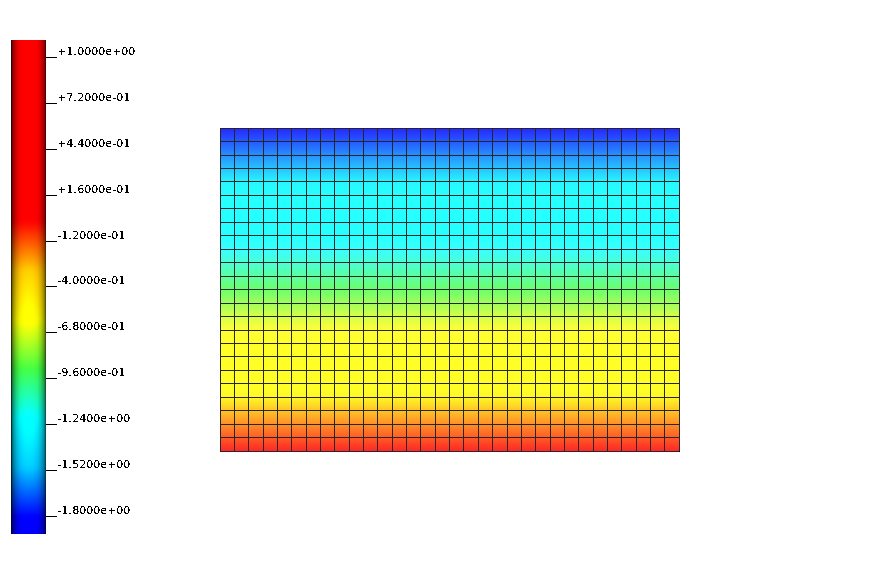
\includegraphics[width=0.9\columnwidth]{examples/example-0101/doc/figures/l160x120x000_n32x24x00_i1_s0.png} 
    \caption{Results, iron $2D$ fine mesh.}
    \label{example-0101-iron-2D-fig}
\end{figure}
%
\begin{figure}[h!]
    \centering 
    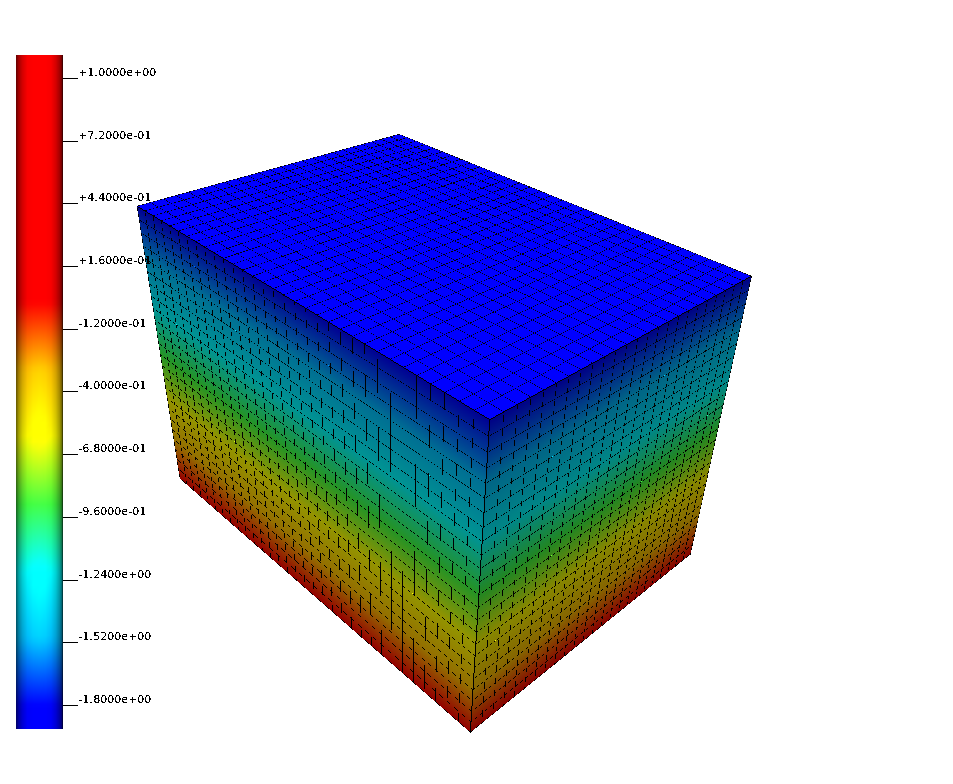
\includegraphics[width=0.9\columnwidth]{examples/example-0101/doc/figures/l160x120x120_n32x24x24_i1_s0.png} 
    \caption{Results, iron $3D$ fine mesh.}
    \label{example-0101-iron-3D-fig}
\end{figure}
%
%===============================================================================
%
\subsubsection{Validation}
%
The iron results are compared to those from Abaqus (version 2017). The figures below show selected results from the validation simulations carried out in Abaqus and provide a qualitative validation. A quantitative validation was carried out by comparing the horizontal displacement $u_y$ along the free-edge ($y=120$ for 2D and $y=z=120$ for 3D) and computing the L2-norm accodring to
\begin{align}
    L_2\texttt{-norm} = \frac{1}{N} \times  \sum_{i=1}^{N} \sqrt{\left(u_{y,\texttt{abaqus}}^i-u_{y,\texttt{iron}}^i  \right)^2},
\end{align}
where $N$ is the total number of nodes along the free-edge. The results over the mesh refinements are given in Table \ref{tab:example-0101-valid-Iron-Abaqus}.
%
\begin{figure}[h!]
    \centering 
    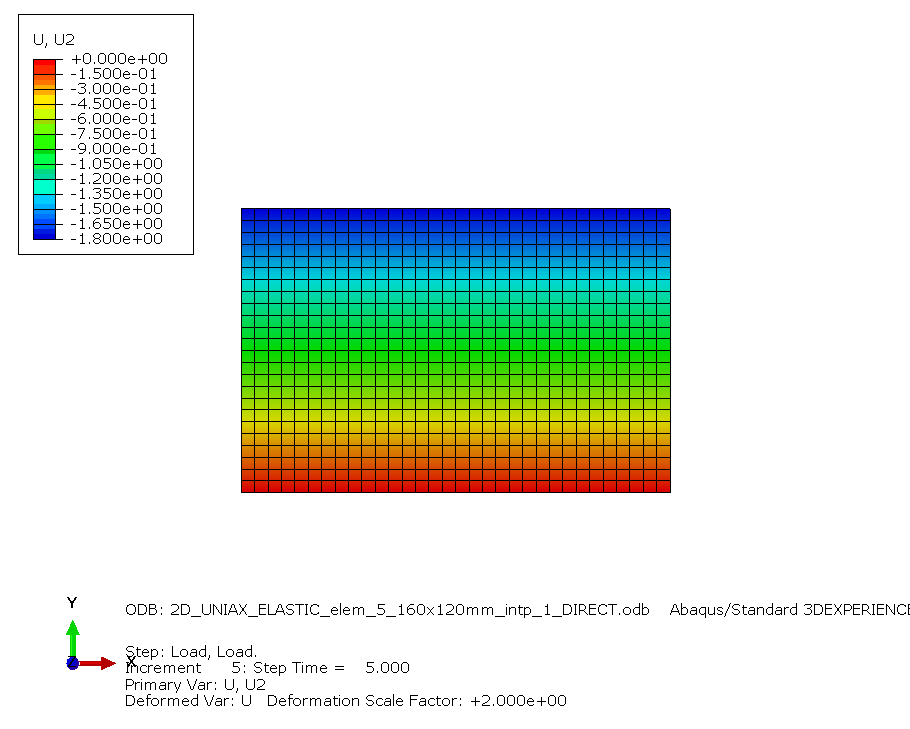
\includegraphics[width=\columnwidth]{examples/example-0101/doc/figures/2D_UNIAX_ELASTIC_elem_5_160x120mm_intp_1_DIRECTU2.png} 
    \caption{Results, Abaqus $2D$ fine mesh.}
    \label{example-0101-abaqus-2D-fig}
\end{figure}
%
\begin{figure}[h!]
    \centering 
    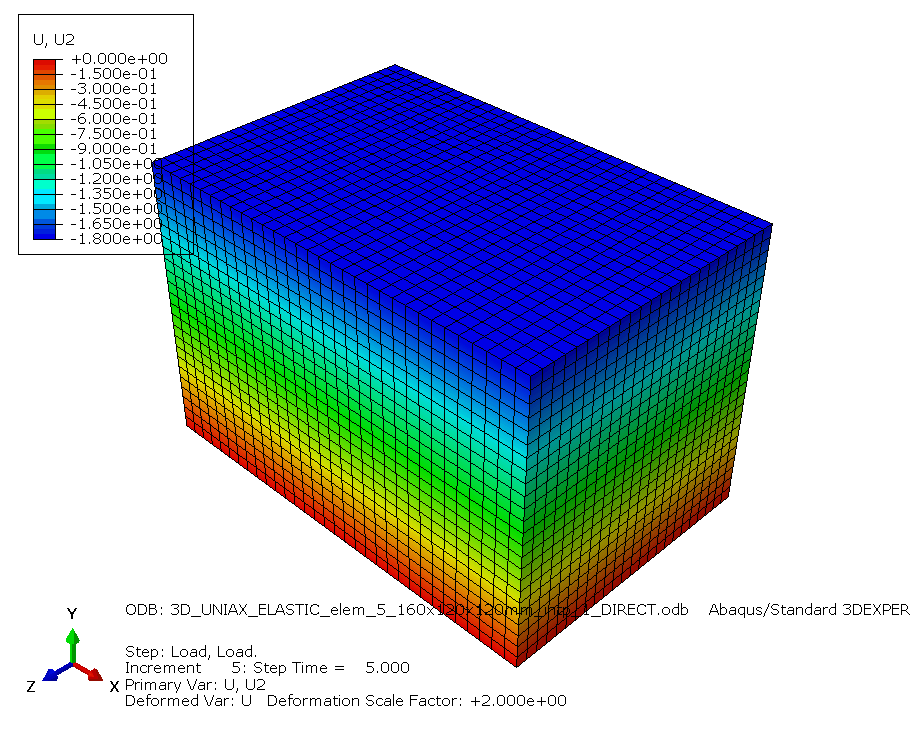
\includegraphics[width=\columnwidth]{examples/example-0101/doc/figures/3D_UNIAX_ELASTIC_elem_5_160x120x120mm_intp_1_DIRECTU2.png} 
    \caption{Results, abaqus $3D$ fine mesh.}
    \label{example-0101-abaqus-3D-fig}
\end{figure}
%
\begin{table}[h!]
	\centering
    \begin{tabular}{llll}
    Dimension & Mesh 		& $L_2\texttt{-norm}$			& Interpolation \\ \hline
    $2D$      & Coarse 	& $5.322\times 10^{-16}$	& Linear \\
    $2D$      & Medium  & $1.559\times 10^{-15}$	& Linear \\
    $2D$      & Fine  	& $2.900\times 10^{-15}$	& Linear \\
    $3D$      & Coarse  & $3.071\times 10^{-17}$	& Linear \\
    $3D$      & Medium  & $2.125\times 10^{-17}$	& Linear \\
		$3D$			&	Fine 		&	$2.924\times 10^{-17}$	& Linear \\
    $2D$      & Coarse 	& $9.728\times 10^{-16}$	& Quadratic \\
    $2D$      & Medium  & $2.039\times 10^{-15}$	& Quadratic \\
    $2D$      & Fine  	& $2.159\times 10^{-15}$	& Quadratic \\
    $3D$      & Coarse  & $6.687\times 10^{-16}$	& Quadratic \\
    $3D$      & Medium  & \ldots									& Quadratic \\
		$3D$			&	Fine 		&	\ldots									& Quadratic \\		
    \end{tabular}
		\caption{Quantiative error between Abaqus 2017 and iron simulations for linear elastic uniaxial extenions}
		\label{tab:example-0101-valid-Iron-Abaqus}
\end{table}
%===============================================================================
%===============================================================================

%
%===============================================================================
%===============================================================================
%
\clearpage
%
\subsection{Example-0101}
%
%===============================================================================
%
\subsubsection{Mathematical model}
%
We solve the following equation,
%
\begin{align}
    \nabla \cdot \boldsymbol{\sigma} (\boldsymbol{u}, t) = \boldsymbol{0} & &&\Omega = [0, 160] \times [0, 120], t \in [0, 5],
\end{align}
%
with time step size $\Delta_t = 1$ and boundary conditions
%
\begin{align}
    \ldots & && \ldots, \\
    \ldots & && \ldots.
\end{align}
%
2D: specify thickness, Young's modulus and Poisson's ratio.
%
%===============================================================================
%
\subsubsection{Computational model}
%
\begin{itemize}
    \item{Length, width, height}
    \item{Direct/iterative solver}
    \item{Generated/user mesh}
    \item{Number of elements}
    \item{Interpolation order}
    \item{Number of solver steps (time steps, load steps)}
\end{itemize}
%
%===============================================================================
%
\subsubsection{Results}
%
\begin{figure}[h!]
    \centering 
    \includegraphics[width=\columnwidth]{examples/example-0101/doc/figures/analytical_solution.eps} 
    \caption{Results, analytical solution.}
    \label{example-0101-analytical-solution-fig}
\end{figure}
%
\begin{figure}[h!]
    \centering 
    \includegraphics[width=\columnwidth]{examples/example-0101/doc/figures/abaqus_reference.eps} 
    \caption{Results, Abaqus reference.}
    \label{example-0101-abaqus-reference-fig}
\end{figure}
%
\begin{figure}[h!]
    \centering 
    \includegraphics[width=\columnwidth]{examples/example-0101/doc/figures/iron_reference.eps} 
    \caption{Results, iron reference.}
    \label{example-0101-iron-reference-fig}
\end{figure}
%
\begin{figure}[h!]
    \centering 
    \includegraphics[width=\columnwidth]{examples/example-0101/doc/figures/current_run.eps} 
    \caption{Results, current run.}
    \label{example-0101-current-run-fig}
\end{figure}
%
%===============================================================================
%
\subsubsection{Validation}
%
CHeart rev.\ 6328, Abaqus 2017, analytical reference solution, whatever...
%
%===============================================================================
%===============================================================================

%
%===============================================================================
%===============================================================================
%
\clearpage
%
\subsection{Example-0111 \texttt{[PLAUSIBLE]}}
%
%===============================================================================
%
\subsubsection{Mathematical model}
%
We solve the following equation (both $2D$ and $3D$ domains are considered),
%
\begin{align}
    \nabla \cdot \boldsymbol{\sigma} (\boldsymbol{u}, t) = \boldsymbol{f} (\boldsymbol{u}, t) & &&\Omega = [0, 160] \times [0, 120] \times [0, 120], t \in [0, 5],
\end{align}
%
with time step size $\Delta_t = 1$ and $\boldsymbol{u} = [u_x,u_y]$ in $2D$ $\boldsymbol{u} = [u_x,u_y,u_z]$ in 3D. The boundary conditions in $2D$ are given by
%
\begin{align}
    u_x = u_y = 0 & &&x = y = 0, \\
		\boldsymbol{f} (u_x) = 6.0 \times 10^{4} & &&x = 160,
\end{align}
%
and in 3D by
\begin{align}
    u_x = u_y = u_z =0 & &&x = y = z =0, \\
		\boldsymbol{f} (u_x) = 7.2 \times 10^{6} & &&x = 160.
\end{align}
The material parameters are
\begin{align}
    E = & 10000\texttt{MPa}, \\
    \nu = & 0.3, \\
		\rho = & 5 \times 10^{-9}\texttt{tonne.mm$^3$}.
\end{align}
%
%===============================================================================
%
\subsubsection{Computational model}
%
\begin{itemize}
    \item{Commandline arguments are:}
        \subitem{float: length along x-direction}
        \subitem{float: length along y-direction}
        \subitem{float: length along z-direction (set to zero for 2D)}
        \subitem{integer: number of elements in x-direction}
        \subitem{integer: number of elements in y-direction}
        \subitem{integer: number of elements in z-direction (set to zero for 2D)}
        \subitem{integer: interpolation order (1: linear; 2: quadratic)}
        \subitem{integer: solver type (0: direct; 1: iterative)}
				\subitem{float: elastic modulus}
				\subitem{float: Poisson ratio}
				\subitem{float: XXX}
    \item{Command line arguments for tests are:}
        \subitem{160 120 0 8 6 0 1 0 10000 0.3 XXX}
				\subitem{160 120 0 16 12 0 1 0 10000 0.3 XXX}
				\subitem{160 120 0 32 24 0 1 0 10000 0.3 XXX}
				\subitem{160 120 120 8 6 6 1 0 10000 0.3 XXX}
				\subitem{160 120 120 16 12 12 1 0 10000 0.3 XXX}
				\subitem{160 120 120 32 24 24 1 0 10000 0.3 XXX}
        \subitem{160 120 0 8 6 0 2 0 10000 0.3 XXX}
				\subitem{160 120 0 16 12 0 2 0 10000 0.3 XXX}
				\subitem{160 120 0 32 24 0 2 0 10000 0.3 XXX}
				\subitem{160 120 120 8 6 6 2 0 10000 0.3 XXX}
				\subitem{160 120 120 16 12 12 2 0 10000 0.3 XXX}
				\subitem{160 120 120 32 24 24 2 0 10000 0.3 XXX}				
\end{itemize}
%
%===============================================================================
%
\subsubsection{Results}
%
\begin{figure}[h!]
    \centering 
    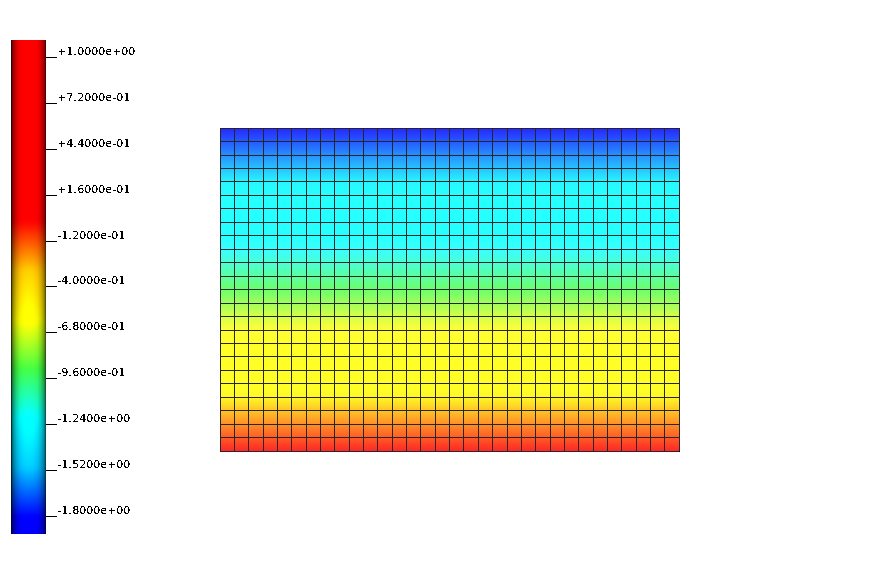
\includegraphics[width=0.9\columnwidth]{examples/example-0101/doc/figures/l160x120x000_n32x24x00_i1_s0.png} 
    \caption{Results, iron $2D$ fine mesh.}
    \label{example-0101-iron-2D-fig}
\end{figure}
%
\begin{figure}[h!]
    \centering 
    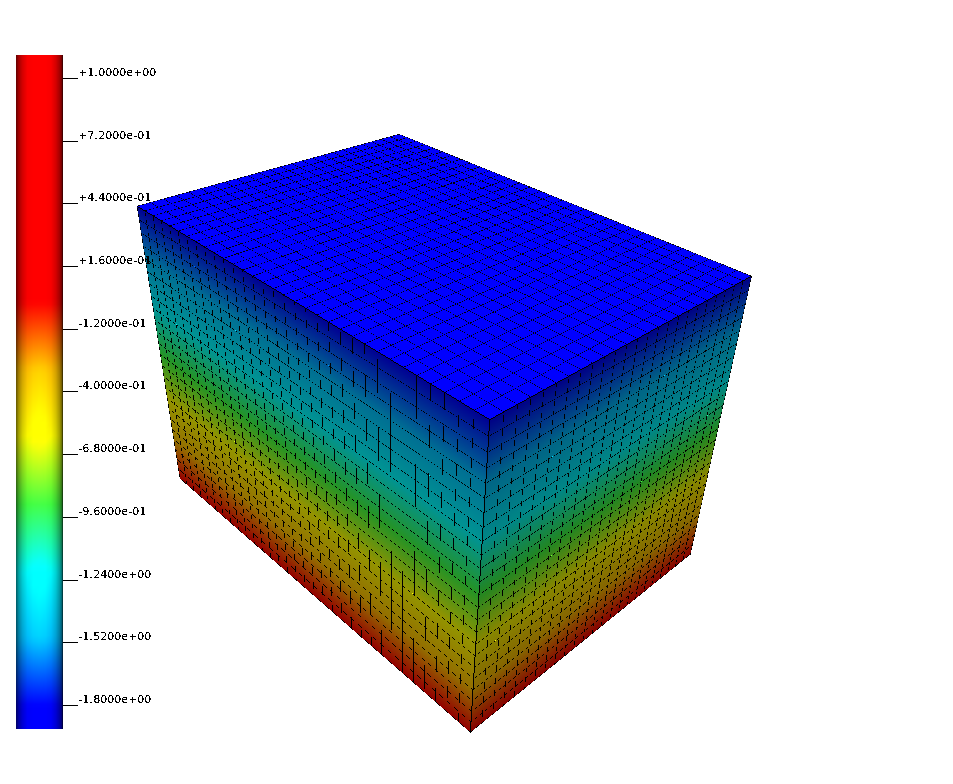
\includegraphics[width=0.9\columnwidth]{examples/example-0101/doc/figures/l160x120x120_n32x24x24_i1_s0.png} 
    \caption{Results, iron $3D$ fine mesh.}
    \label{example-0101-iron-3D-fig}
\end{figure}
%
%===============================================================================
%
\subsubsection{Validation}
%
The iron results are compared to those from Abaqus (version 2017). The figures below show selected results from the validation simulations carried out in Abaqus and provide a qualitative validation. A quantitative validation was carried out by comparing the horizontal displacement $u_y$ along the free-edge ($y=120$ for 2D and $y=z=120$ for 3D) and computing the L2-norm accodring to
\begin{align}
    L_2\texttt{-norm} = \frac{1}{N} \times  \sum_{i=1}^{N} \sqrt{\left(u_{y,\texttt{abaqus}}^i-u_{y,\texttt{iron}}^i  \right)^2},
\end{align}
where $N$ is the total number of nodes along the free-edge. The results over the mesh refinements are given in Table \ref{tab:example-0101-valid-Iron-Abaqus}.
%
\begin{figure}[h!]
    \centering 
    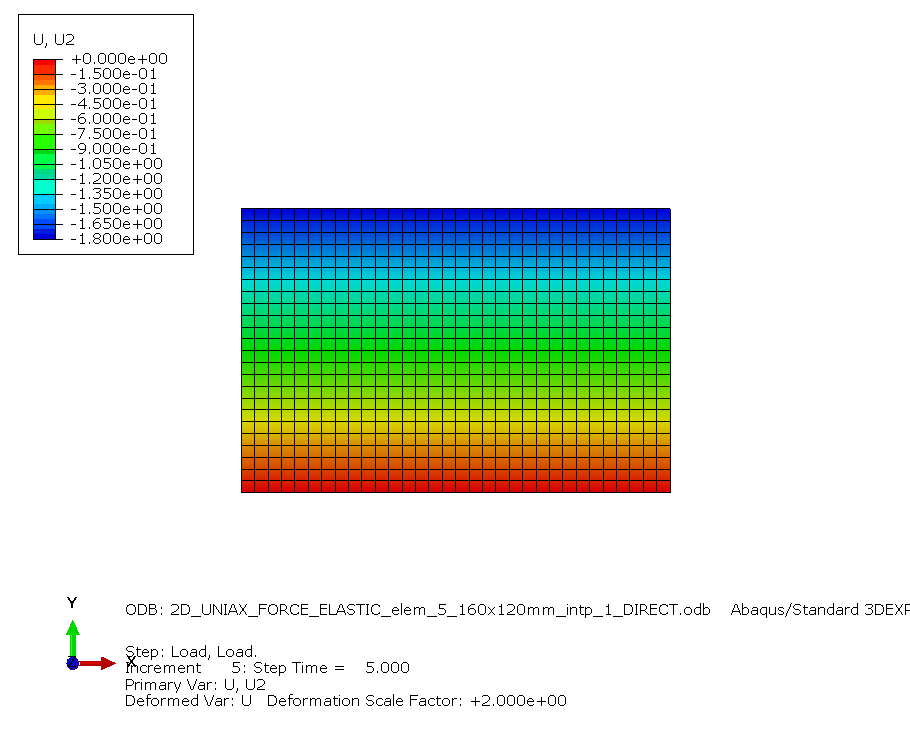
\includegraphics[width=\columnwidth]{examples/example-0111/doc/figures/2D_UNIAX_FORCE_ELASTIC_elem_5_160x120mm_intp_1_DIRECTU2.png} 
    \caption{Results, Abaqus $2D$ fine mesh.}
    \label{example-0101-abaqus-2D-fig}
\end{figure}
%
\begin{figure}[h!]
    \centering 
    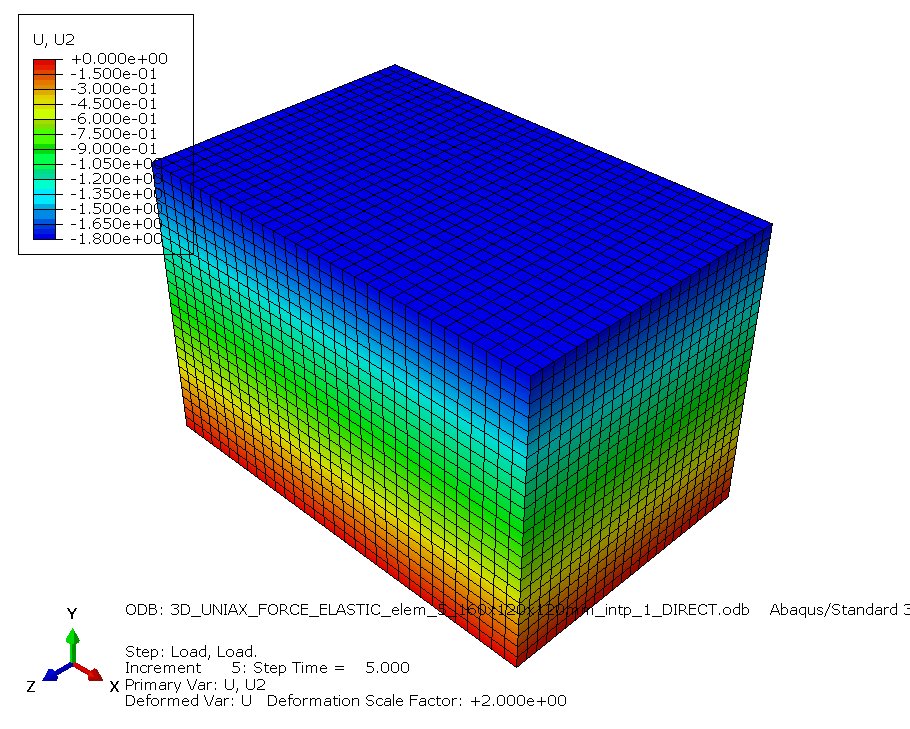
\includegraphics[width=\columnwidth]{examples/example-0111/doc/figures/3D_UNIAX_FORCE_ELASTIC_elem_5_160x120x120mm_intp_1_DIRECTU2.png} 
    \caption{Results, abaqus $3D$ fine mesh.}
    \label{example-0101-abaqus-3D-fig}
\end{figure}
%
\begin{table}[h!]
	\centering
    \begin{tabular}{llll}
    Dimension & Mesh 		& $L_2\texttt{-norm}$			& Interpolation \\ \hline
    $2D$      & Coarse 	& \ldots									& Linear \\
    $2D$      & Medium  & \ldots									& Linear \\
    $2D$      & Fine  	& \ldots									& Linear \\
    $3D$      & Coarse  & \ldots									& Linear \\
    $3D$      & Medium  & \ldots									& Linear \\
		$3D$			&	Fine 		&	\ldots									& Linear \\
    $2D$      & Coarse 	& \ldots									& Quadratic \\
    $2D$      & Medium  & \ldots									& Quadratic \\
    $2D$      & Fine  	& \ldots									& Quadratic \\
    $3D$      & Coarse  & \ldots									& Quadratic \\
    $3D$      & Medium  & \ldots									& Quadratic \\
		$3D$			&	Fine 		&	\ldots									& Quadratic \\		
    \end{tabular}
		\caption{Quantiative error between Abaqus 2017 and iron simulations for linear elastic uniaxial extenions}
		\label{tab:example-0101-valid-Iron-Abaqus}
\end{table}
%===============================================================================
%===============================================================================

%
%===============================================================================
%===============================================================================
%
\clearpage
%
\subsection{Example-0112 \texttt{[CONVERGES]}}
%
%===============================================================================
%
\subsubsection{Mathematical model}
%
We solve the following equation,
%
\begin{align}
    \nabla \cdot \boldsymbol{\sigma} (\boldsymbol{u}, t) = \boldsymbol{0} & &&\Omega = [0, 160] \times [0, 120], t \in [0, 5],
\end{align}
%
with time step size $\Delta_t = 1$ and boundary conditions
%
\begin{align}
    \ldots & && \ldots, \\
    \ldots & && \ldots.
\end{align}
%
2D: specify thickness, Young's modulus and Poisson's ratio.
%
%===============================================================================
%
\subsubsection{Computational model}
%
\begin{itemize}
    \item{Length, width, height}
    \item{Direct/iterative solver}
    \item{Generated/user mesh}
    \item{Number of elements}
    \item{Interpolation order}
    \item{Number of solver steps (time steps, load steps)}
\end{itemize}
%
%===============================================================================
%
\subsubsection{Results}
%
\begin{figure}[h!]
    \centering 
    \includegraphics[width=\columnwidth]{examples/example-0101/doc/figures/analytical_solution.eps} 
    \caption{Results, analytical solution.}
    \label{example-0101-analytical-solution-fig}
\end{figure}
%
\begin{figure}[h!]
    \centering 
    \includegraphics[width=\columnwidth]{examples/example-0101/doc/figures/abaqus_reference.eps} 
    \caption{Results, Abaqus reference.}
    \label{example-0101-abaqus-reference-fig}
\end{figure}
%
\begin{figure}[h!]
    \centering 
    \includegraphics[width=\columnwidth]{examples/example-0101/doc/figures/iron_reference.eps} 
    \caption{Results, iron reference.}
    \label{example-0101-iron-reference-fig}
\end{figure}
%
\begin{figure}[h!]
    \centering 
    \includegraphics[width=\columnwidth]{examples/example-0101/doc/figures/current_run.eps} 
    \caption{Results, current run.}
    \label{example-0101-current-run-fig}
\end{figure}
%
%===============================================================================
%
\subsubsection{Validation}
%
CHeart rev.\ 6328, Abaqus 2017, analytical reference solution, whatever...
%
%===============================================================================
%===============================================================================

%===============================================================================
%
\clearpage
%
\section{Finite elasticity}
%
%%===============================================================================
%===============================================================================
%
\clearpage
%
\subsection{Example-0004 \texttt{[VALIDATED]}}
%
Example uses generated regular meshes and solves a static problem, i.e., applies
the boundary conditions in one step.
%
%===============================================================================
%
\subsubsection{Mathematical model - 2D}
%
We solve the following scalar equation,
%
\begin{align}
    \nabla \cdot \nabla u = 0 & &&\Omega = [0, 2] \times [0, 1],
\end{align}
%
with boundary conditions
%
\begin{align}
    u = 2.0 e^x \cdot cos(y)    & &&\text{on } \partial\Omega.
\end{align}
%
No material parameters to specify.
%
%===============================================================================
%
\subsubsection{Computational model}
%
\begin{itemize}
    \item{Commandline arguments are:}
        \subitem{integer: number of elements in x-direction}
        \subitem{integer: number of elements in y-direction}
        \subitem{integer: number of elements in z-direction (set to zero for 2D)}
        \subitem{interger: interpolation order (1: linear; 2: quadratic)}
        \subitem{integer: solver type (0: direct; 1: iterative)}
    \item{Commandline arguments for tests are:}
        \subitem{4 2 0 1 0}
        \subitem{8 4 0 1 0}
        \subitem{2 1 0 2 0}
        \subitem{4 2 0 2 0}
        \subitem{8 4 0 2 0}
        \subitem{4 2 0 1 1}
        \subitem{8 4 0 1 1}
        \subitem{2 1 0 2 1}
        \subitem{4 2 0 2 1}
        \subitem{8 4 0 2 1}
        \subitem{100 50 0 1 0 (not tested yet..)}
        \subitem{100 50 0 2 0 (not tested yet..)}
        \subitem{100 50 0 1 1 (not tested yet..)}
        \subitem{100 50 0 2 1 (not tested yet..)}
\end{itemize}
%
%===============================================================================
%
\subsubsection{Result summary}
%
We use CHeart rev.\ 6292 to produce numerical reference solutions.
%
\verbatiminput{examples/example-0004/results/results.summary}
\verbatiminput{examples/example-0004/results/failed.tests}
%
\begin{figure}[h!]
    \centering 
    \includegraphics[width=0.9\columnwidth]{examples/example-0004/doc/figures/iron_reference_2D.eps} 
    \caption{2D results, iron reference w/ command line arguments [8 4 0 2 0].}
    \label{example-0004-iron-2D-reference-fig}
\end{figure}
%
\begin{figure}[h!]
    \centering 
    \includegraphics[width=0.9\columnwidth]{examples/example-0004/doc/figures/current_run_l4x2x0_n8x4x0_i2_s0.eps} 
    \caption{2D results, current run w/ command line arguments [8 4 0 2 0].}
    \label{example-0004-current-run-2D-fig}
\end{figure}
%
%===============================================================================
%===============================================================================

%
%===============================================================================
%
\clearpage
%
\section{Navier-Stokes flow}
%
\subsection{Equation in general form}
%
\begin{equation}
    \partial_{t} (\rho \boldsymbol{v}) + \nabla \cdot (\rho \boldsymbol{v} \otimes \boldsymbol{v} + p \boldsymbol{I}) = \rho \boldsymbol{f}
\end{equation}
%
%%===============================================================================
%===============================================================================
%
\clearpage
%
\subsection{Example-0004 \texttt{[VALIDATED]}}
%
Example uses generated regular meshes and solves a static problem, i.e., applies
the boundary conditions in one step.
%
%===============================================================================
%
\subsubsection{Mathematical model - 2D}
%
We solve the following scalar equation,
%
\begin{align}
    \nabla \cdot \nabla u = 0 & &&\Omega = [0, 2] \times [0, 1],
\end{align}
%
with boundary conditions
%
\begin{align}
    u = 2.0 e^x \cdot cos(y)    & &&\text{on } \partial\Omega.
\end{align}
%
No material parameters to specify.
%
%===============================================================================
%
\subsubsection{Computational model}
%
\begin{itemize}
    \item{Commandline arguments are:}
        \subitem{integer: number of elements in x-direction}
        \subitem{integer: number of elements in y-direction}
        \subitem{integer: number of elements in z-direction (set to zero for 2D)}
        \subitem{interger: interpolation order (1: linear; 2: quadratic)}
        \subitem{integer: solver type (0: direct; 1: iterative)}
    \item{Commandline arguments for tests are:}
        \subitem{4 2 0 1 0}
        \subitem{8 4 0 1 0}
        \subitem{2 1 0 2 0}
        \subitem{4 2 0 2 0}
        \subitem{8 4 0 2 0}
        \subitem{4 2 0 1 1}
        \subitem{8 4 0 1 1}
        \subitem{2 1 0 2 1}
        \subitem{4 2 0 2 1}
        \subitem{8 4 0 2 1}
        \subitem{100 50 0 1 0 (not tested yet..)}
        \subitem{100 50 0 2 0 (not tested yet..)}
        \subitem{100 50 0 1 1 (not tested yet..)}
        \subitem{100 50 0 2 1 (not tested yet..)}
\end{itemize}
%
%===============================================================================
%
\subsubsection{Result summary}
%
We use CHeart rev.\ 6292 to produce numerical reference solutions.
%
\verbatiminput{examples/example-0004/results/results.summary}
\verbatiminput{examples/example-0004/results/failed.tests}
%
\begin{figure}[h!]
    \centering 
    \includegraphics[width=0.9\columnwidth]{examples/example-0004/doc/figures/iron_reference_2D.eps} 
    \caption{2D results, iron reference w/ command line arguments [8 4 0 2 0].}
    \label{example-0004-iron-2D-reference-fig}
\end{figure}
%
\begin{figure}[h!]
    \centering 
    \includegraphics[width=0.9\columnwidth]{examples/example-0004/doc/figures/current_run_l4x2x0_n8x4x0_i2_s0.eps} 
    \caption{2D results, current run w/ command line arguments [8 4 0 2 0].}
    \label{example-0004-current-run-2D-fig}
\end{figure}
%
%===============================================================================
%===============================================================================

%
%===============================================================================
%===============================================================================
%
\clearpage
%
\subsection{Example-0302-u \texttt{[COMPILES]}}
%
Example uses user-defined simplex meshes in CHeart mesh format with
quadratic/linear interpolation for velocity/pressure
and solves a dynamic problem.

Setup is the well-known lid-driven cavity problem
on the unit square or unit cube in two and three dimensions.

Current issue: does not converge after 30 some time iterations.
%
%===============================================================================
%
\subsubsection{Mathematical model - 2D}
%
We solve the incompressible Navier-Stokes equation,
%
\begin{align}
    \partial_{t} (\rho \boldsymbol{v}) + \nabla \cdot (\rho \boldsymbol{v} \otimes \boldsymbol{v}) - \nabla \cdot (\mu \nabla \boldsymbol{v} - p \boldsymbol{I}) = \rho \boldsymbol{f} & &&\Omega = [0, 1] \times [0, 1], \\
    \nabla \cdot \boldsymbol{v} = 0,
\end{align}
%
with boundary conditions
%
\begin{align}
    \boldsymbol{v} &= 0         &&x = 0, \\
    \boldsymbol{v} &= 0         &&x = 1, \\
    \boldsymbol{v} &= 0         &&y = 0, \\
    \boldsymbol{v} &= [1, 0]^T  &&y = 1.
\end{align}
%
Viscosity $\mu = 0.0025$, density $\rho = 1$. Thus, Reynolds number $Re = 400$.
%
%===============================================================================
%
\subsubsection{Mathematical model - 3D}
%
We solve the incompressible Navier-Stokes equation,
%
\begin{align}
    \partial_{t} (\rho \boldsymbol{v}) + \nabla \cdot (\rho \boldsymbol{v} \otimes \boldsymbol{v}) - \nabla \cdot (\mu \nabla \boldsymbol{v} - p \boldsymbol{I}) = \rho \boldsymbol{f} & &&\Omega = [0, 1] \times [0, 1] \times [0, 1], \\
    \nabla \cdot \boldsymbol{v} = 0,
\end{align}
%
with boundary conditions
%
\begin{align}
    \boldsymbol{v} &= 0         &&x = 0, \\
    \boldsymbol{v} &= 0         &&x = 1, \\
    \boldsymbol{v} &= 0         &&y = 0, \\
    \boldsymbol{v} &= [1, 0]^T  &&y = 1, \\
    \boldsymbol{v} &= 0         &&z = 0, \\
    \boldsymbol{v} &= 0         &&z = 1.
\end{align}
%
Viscosity $\mu = 0.0025$, density $\rho = 1$. Thus, Reynolds number $Re = 100$.
%
%===============================================================================
%
\subsubsection{Computational model}
%
\begin{itemize}
    \item{Commandline arguments are:}
        \subitem{integer: number of dimensions (2: 2D, 3: 3D}
        \subitem{integer: mesh refinement level (1, 2, 3, ...)}
        \subitem{float: start time}
        \subitem{float: stop time}
        \subitem{float: time step size}
        \subitem{float: density}
        \subitem{float: viscosity}
        \subitem{integer: solver type (0: direct; 1: iterative)}
    \item{Commandline arguments for tests are:}
        \subitem{2 1 0.0 0.01 0.001 1.0 0.0025 0}
    \item{Note: Binary uses command line arguments to search for the relevant mesh files.}
\end{itemize}
%
%===============================================================================
%
\subsubsection{Result summary}
%
We use CHeart rev.\ 6292 to produce numerical reference solutions.
%
\verbatiminput{examples/example-0302-u/results/results.summary}
\verbatiminput{examples/example-0302-u/results/failed.tests}
%
%\begin{figure}[h!]
%%    \centering 
%    \includegraphics[width=0.9\columnwidth]{examples/example-0302-u/doc/figures/iron_reference_2D.eps} 
%    \caption{2D results, iron reference w/ command line arguments [2.0 1.0 0.0 8 4 0 1 0].}
%    \label{example-0302-u-iron-2D-reference-fig}
%\end{figure}
%%
%\begin{figure}[h!]
%    \centering 
%    \includegraphics[width=0.9\columnwidth]{examples/example-0302-u/doc/figures/current_run_l2x1x0_n8x4x0_i1_s0.eps} 
%    \caption{2D results, current run w/ command line arguments [2.0 1.0 0.0 8 4 0 1 0].}
%    \label{example-0302-u-current-run-2D-fig}
%\end{figure}
%%
%\begin{figure}[h!]
%    \centering 
%    \includegraphics[width=0.9\columnwidth]{examples/example-0302-u/doc/figures/iron_reference_3D.eps} 
%    \caption{3D results, iron reference w/ command line arguments [2.0 1.0 1.0 8 4 4 1 0].}
%    \label{example-0302-u-iron-3D-reference-fig}
%\end{figure}
%%
%\begin{figure}[h!]
%    \centering 
%    \includegraphics[width=0.9\columnwidth]{examples/example-0302-u/doc/figures/current_run_l2x1x1_n8x4x4_i1_s0.eps} 
%    \caption{3D results, current run w/ command line arguments [2.0 1.0 1.0 8 4 4 1 0].}
%    \label{example-0302-u-current-run-3D-fig}
%\end{figure}
%
%===============================================================================
%===============================================================================

%
%===============================================================================
%
\clearpage
%
\section{Monodomain}
%
%%===============================================================================
%===============================================================================
%
\clearpage
%
\subsection{Example-0401 \texttt{[PLAUSIBLE]}}
%
%===============================================================================
%
\subsubsection{Mathematical model}
%
We solve the Monodomain Equation
%
\begin{align}
    \sigma \Delta V_m(t) = A_m\Big(C_m \dfrac{\partial V_m}{\partial t} + I_{ionic}(V_m)\Big) & &&\Omega = [0, 1] \times [0, 1], \quad t \in [0, 3.0]
\end{align}
%
where $V_m(t)$ is given by the Hodgkin-Huxley system of ODEs \cite{hodgkin1952propagation}

with boundary conditions
%
\begin{align}
    V_m = 0 & &&x = y = 0, \\
    V_m = 0 & &&x = y = 1.
\end{align}
and initial values
%
\begin{equation*}
  \begin{array}{lll}
    V_m(t=0) = -75
  \end{array}
\end{equation*}
%
Additionally a stimulation current $I_{stim}$ is applied for $t_{stim} = [0, 0.1]$ at the center node of the domain (i.e. at $(x,y) = (\frac12, \frac12,)$).
%

Material parameters:
\begin{equation*}
  \begin{array}{lll}
    \sigma = 3.828\\[4mm]
    A_m = 500\\[4mm]
    C_m = 0.58 \quad \text{for the slow-twitch case,} \quad C_m = 1.0 \quad \text{for the fast-twitch case}\\[4mm]
    I_{Stim} = 1200 \quad \text{for the slow-twitch case,} \quad I_{Stim} = 2000.0 \quad \text{for the fast-twitch case}\\[4mm]
  \end{array}
\end{equation*}
%
%===============================================================================
%
\subsubsection{Computational model}
%
\begin{itemize}
    \item{This example uses generated meshes}
    \item{Commandline arguments are:}
        \subitem{number elements X} 		
        \subitem{number elements Y}		
        \subitem{interpolation order (1: linear; 2: quadratic)}
        \subitem{solver type (0: direct; 1: iterative)}	
        \subitem{PDE step size}
        \subitem{stop time}
        \subitem{output frequency} 		
        \subitem{CellML Model URL}
        \subitem{slow-twitch}	
        \subitem{ODE time-step}
    \item{Commands for tests are:}
     \subitem{\verb|./folder/src/example 24 24 1 0 0.005 3.0 1 hodgkin_huxley_1952.cellml F 0.0001|}
     \subitem{\verb|./folder/src/example 24 24 1 0 0.005 3.0 1 hodgkin_huxley_1952.cellml F 0.005|}
     \subitem{\verb|./folder/src/example 10 10 1 0 0.005 3.0 1 hodgkin_huxley_1952.cellml F 0.0001|}
     \subitem{\verb|mpirun -n 2 ./folder/src/example 24 24 1 0 0.005 3.0 1 hodgkin_huxley_1952.cellml F 0.0001|}
     \subitem{\verb|mpirun -n 8 ./folder/src/example 24 24 1 0 0.005 3.0 1 hodgkin_huxley_1952.cellml F 0.0001|}
     \subitem{\verb|./folder/src/example 2 2 1 0 0.005 3.0 1 hodgkin_huxley_1952.cellml F 0.0001|}
     \subitem{\verb|mpirun -n 2 ./folder/src/example 2 2 1 0 0.005 3.0 1 hodgkin_huxley_1952.cellml F 0.0001|}
    \item{This is a dynamic problem.}
\end{itemize}
%
%===============================================================================
%
\subsubsection{Results}
%
\verbatiminput{examples/example-0401/results/results.summary}
\verbatiminput{examples/example-0401/results/failed.tests}
%

\begin{figure}[ht]
  \centering
  \includegraphics[width=0.9\columnwidth]{examples/example-0401/doc/figures/current_run_l1x1_n10x10_i1_s0_p1__t20.png}
  \caption{Result of scenario with $10 \times 10$ elements, $t=20$, direct solver, $p=1$ process}
  \label{example-0401-current-run1-fig}
\end{figure}

\begin{figure}[ht]
  \centering
  \includegraphics[width=0.9\columnwidth]{examples/example-0401/doc/figures/current_run_l1x1_n24x24_i1_s0_p1__t20.png}
  \caption{Result of scenario with $24 \times 24$ elements, $t=20$, direct solver, $p=1$ process}
  \label{example-0401-current-run2-fig}
\end{figure}

\begin{figure}[ht]
  \centering
  \includegraphics[width=0.9\columnwidth]{examples/example-0401/doc/figures/current_run_l1x1_n24x24_i1_s1_p1__t20.png}
  \caption{Result of scenario with $24 \times 24$ elements, $t=20$, iterative solver, $p=1$ process}
  \label{example-0401-current-run3-fig}
\end{figure}

\begin{figure}[ht]
  \centering
  \includegraphics[width=0.9\columnwidth]{examples/example-0401/doc/figures/current_run_l1x1_n24x24_i1_s0_p2__t41.png}
  \caption{Result of scenario with $24 \times 24$ elements, $t=20$, iterative solver, $p=2$ processes}
  \label{example-0401-current-run4-fig}
\end{figure}

\begin{figure}[ht]
  \centering
  \includegraphics[width=0.9\columnwidth]{examples/example-0401/doc/figures/current_run_l1x1_n24x24_i1_s0_p8__t167.png}
  \caption{Result of scenario with $24 \times 24$ elements, $t=20$, iterative solver, $p=8$ processes}
  \label{example-0401-current-run5-fig}
\end{figure}

\begin{figure}[ht]
  \centering
  \includegraphics[width=0.9\columnwidth]{examples/example-0401/doc/figures/current_run_l1x1_n2x2_i1_s0_p1__t20.png}
  \caption{Result of scenario with $2 \times 2$ elements, $t=20$, direct solver, $p=1$ process}
  \label{example-0401-current-run6-fig}
\end{figure}

\begin{figure}[ht]
  \centering
  \includegraphics[width=0.9\columnwidth]{examples/example-0401/doc/figures/current_run_l1x1_n2x2_i1_s0_p2__t41.png}
  \caption{Result of scenario with $2 \times 2$ elements, $t=20$, direct solver, $p=2$ processes}
  \label{example-0401-current-run7-fig}
\end{figure}

With the 'big' target there will be animations created. You get a better understanding of the solutions by looking at them in \verb|iron-tests/examples/example-0401/doc/figures|.

%===============================================================================
%
\subsubsection{Validation}
%
We compare with a Matlab implementation as well as with reference iron files.

The matlab scripts use finite difference discretization instead of finite elements.
The results are qualitatively the same but exactly. The compare script also tests for matlab reference data which is only included for the 2 examples with $24\times 24$ elements. There is a big $L_2$-error. The tolerance is set to a high value to allow for the tests to succeed. With this the comparing-mechanism is tested. Maybe in the future someone succeeds to generate suitable matlab data that then can just be exchanged without having to rewrite the compare script.

The iron files to compare with are the output of the simulation as of Aug. 2017. In that way we can check if the simulation brakes with respect to the current state.
In order to keep file sizes minimal the comparision is only conducted for time steps ${t=0.01, 0.1, 0.2, 1, 2, 3}$ for the 'big' target and ${t=0.1, 0.2, 1}$ for the 'fast' target.
%
%===============================================================================
%===============================================================================

%
%===============================================================================
%
\clearpage
%
\section{CellML model}
%
%%===============================================================================
%===============================================================================
%
\clearpage
%
\subsection{Example-0004 \texttt{[VALIDATED]}}
%
Example uses generated regular meshes and solves a static problem, i.e., applies
the boundary conditions in one step.
%
%===============================================================================
%
\subsubsection{Mathematical model - 2D}
%
We solve the following scalar equation,
%
\begin{align}
    \nabla \cdot \nabla u = 0 & &&\Omega = [0, 2] \times [0, 1],
\end{align}
%
with boundary conditions
%
\begin{align}
    u = 2.0 e^x \cdot cos(y)    & &&\text{on } \partial\Omega.
\end{align}
%
No material parameters to specify.
%
%===============================================================================
%
\subsubsection{Computational model}
%
\begin{itemize}
    \item{Commandline arguments are:}
        \subitem{integer: number of elements in x-direction}
        \subitem{integer: number of elements in y-direction}
        \subitem{integer: number of elements in z-direction (set to zero for 2D)}
        \subitem{interger: interpolation order (1: linear; 2: quadratic)}
        \subitem{integer: solver type (0: direct; 1: iterative)}
    \item{Commandline arguments for tests are:}
        \subitem{4 2 0 1 0}
        \subitem{8 4 0 1 0}
        \subitem{2 1 0 2 0}
        \subitem{4 2 0 2 0}
        \subitem{8 4 0 2 0}
        \subitem{4 2 0 1 1}
        \subitem{8 4 0 1 1}
        \subitem{2 1 0 2 1}
        \subitem{4 2 0 2 1}
        \subitem{8 4 0 2 1}
        \subitem{100 50 0 1 0 (not tested yet..)}
        \subitem{100 50 0 2 0 (not tested yet..)}
        \subitem{100 50 0 1 1 (not tested yet..)}
        \subitem{100 50 0 2 1 (not tested yet..)}
\end{itemize}
%
%===============================================================================
%
\subsubsection{Result summary}
%
We use CHeart rev.\ 6292 to produce numerical reference solutions.
%
\verbatiminput{examples/example-0004/results/results.summary}
\verbatiminput{examples/example-0004/results/failed.tests}
%
\begin{figure}[h!]
    \centering 
    \includegraphics[width=0.9\columnwidth]{examples/example-0004/doc/figures/iron_reference_2D.eps} 
    \caption{2D results, iron reference w/ command line arguments [8 4 0 2 0].}
    \label{example-0004-iron-2D-reference-fig}
\end{figure}
%
\begin{figure}[h!]
    \centering 
    \includegraphics[width=0.9\columnwidth]{examples/example-0004/doc/figures/current_run_l4x2x0_n8x4x0_i2_s0.eps} 
    \caption{2D results, current run w/ command line arguments [8 4 0 2 0].}
    \label{example-0004-current-run-2D-fig}
\end{figure}
%
%===============================================================================
%===============================================================================

%
%
%===============================================================================
%	BIBLIOGRAPHY
%===============================================================================
%===============================================================================
%
\clearpage
%
%\renewcommand{\refname}{\spacedlowsmallcaps{References}} % For modifying the bibliography heading
\bibliographystyle{unsrt}
\bibliography{doc/refs}
%===============================================================================
%===============================================================================
\end{document}
%===============================================================================
%===============================================================================
%===============================================================================
%===============================================================================
